\documentclass[10pt,a4paper,twocolumn]{article}

\usepackage[utf8]{inputenc}
\usepackage[T1]{fontenc}
\usepackage{lmodern}
\usepackage[top=2.2cm,bottom=2.4cm,left=1.8cm,right=1.8cm,columnsep=0.7cm]{geometry}
\usepackage{abstract}
\renewcommand{\abstractnamefont}{\normalfont\small\bfseries}
\renewcommand{\abstracttextfont}{\normalfont\small}
\usepackage{microtype}
\usepackage{booktabs}
\usepackage{tabularx}
\usepackage{graphicx}
\usepackage{pgfplots}
\pgfplotsset{compat=1.17}
\usepackage[numbers,sort&compress]{natbib}
\usepackage{xurl}
\usepackage[hidelinks]{hyperref}
\usepackage{caption}
\captionsetup{font=small,labelfont=bf}

\newcommand{\code}[1]{\texttt{#1}}

\title{Rules First, Models Second: Detecting Personal Data in\\
English, French, German and Luxembourgish Text}

\author{Yann Klees\\
\small \url{https://github.com/YannKleees/tagging}}

\date{November 2026}

\begin{document}
\twocolumn[
\maketitle

\begin{onecolabstract}
\noindent
Documents written in Luxembourg mix four languages and carry identifiers that general tools for
detecting personal data do not know. This paper describes \emph{tagging}, an open source tool that
combines a rule engine written in Rust with two optional models for named entity recognition, and
compares it with Microsoft Presidio on the same data. The rules cover formats with check digits,
word lists from Wikidata, a grammar for names, labelled form fields and addresses. A list of 190{,}000 everyday words, counted from Wikipedia text and taken from the
official Luxembourgish dictionary, removes model output that is no name. On template sentences in
Luxembourg's formats with names the word lists had not been built around, the tool covered 0.93 to
0.97 of all labelled items with a model switched on, against 0.87 for Presidio. On synthetic
letters and forms from another generator it covered 0.75 to 0.84 against 0.49 to 0.59. On text
without personal data it marked 7 to 16 spans where Presidio marked 71 to 115. Presidio remained
ahead on names in German and Luxembourgish Wikipedia sentences (0.87 and 0.83 against 0.85 and
0.77), and it was 18 times faster than the more accurate of the two models. The rules alone found 0.98 of the persons in the first test set and 0.54 once the names were
replaced, which shows how much a saturated test set can hide. All data were synthetic or
encyclopedic, so performance on real documents remains unmeasured.

\medskip\noindent \textbf{Keywords:} personal data, de-identification, named entity recognition,
Luxembourgish, rule-based systems, evaluation
\end{onecolabstract}
\vspace{1.2em}
]
\saythanks

\section{Introduction}

The General Data Protection Regulation asks organisations to limit the personal data they keep and
share \citep{gdpr}. In practice this often means removing names, addresses and identifiers from
text before it is passed on, analysed or sent to a language model. Tools for this task exist. The
best known open source one is Microsoft Presidio \citep{presidio}, which combines pattern
recognisers with a statistical model for named entities.

Such tools are built around large languages and, for identifiers, largely around American
formats. Luxembourg is a hard case for them. Administrative and private text is written in
Luxembourgish, French, German and English, often within one document. Luxembourgish has few
language resources, and no pipeline for it exists in the common libraries. The country has its own
national identification number, the \emph{matricule}, with two check digits, and its own phone and
address conventions. Many residents and cross-border workers also carry French, Belgian or German
identifiers.

A second problem is less often measured. A tool that marks too much is as unusable as one that
marks too little, because a redacted text must remain readable. German and Luxembourgish write
every noun with a capital letter, which removes the cheapest signal that a word is a name.

This paper asks two questions. First, can a system that puts rules first and uses a model only for
what rules cannot know reach the coverage of a general tool on text in Luxembourg's formats, while
marking less of the text that contains no personal data? Second, how far do results on a test set
built by the developer carry over to names and documents the system has not seen? The second
question arose during the work: an early version scored close to 1.00 on its own test set, and the
paper reports what happened when the names in that test set were replaced.

The contributions are a description of the system, an evaluation on four kinds of data with a
strict separation of development and test material, and a comparison with Presidio that states
where each tool is ahead.

\section{Materials and Methods}

\subsection{System}

The system, called \emph{tagging} \citep{tagging}, has a core written in Rust with bindings for
Python and a build for WebAssembly. Each detector returns spans with a type, byte offsets and a
score. Overlapping spans were resolved in favour of the longest and then the highest scoring one,
and spans below a threshold of 0.5 were dropped.

\paragraph{Formats and check digits.} Regular expressions proposed candidates for emails, URLs,
IP addresses, phone numbers, IBANs, payment cards and dates, and each candidate was validated:
IBANs by the ISO 7064 remainder, cards by the Luhn algorithm and issuer prefix, the Luxembourg
matricule by its Luhn and Verhoeff digits. The French social security number, the Belgian national
number and the German pension and tax numbers were validated by their own check digits. Codes
shaped like passport numbers were accepted unless a word such as \emph{order} or \emph{invoice}
preceded them. A date became a date of birth when a birth keyword stood nearby.

\paragraph{Word lists.} First names (4{,}383), family names (19{,}516), places and organisations
were taken from Wikidata \citep{vrandecic2014wikidata}: the given and family names of people with
one of nine citizenships, the localities of Luxembourg, sovereign states, well-known cities and
organisations. Short hand-kept lists added Luxembourgish nicknames and local organisations.

\paragraph{Name grammar.} A first name took the surname after it, a title marked the name after
it, and a company form or a business word turned neighbouring capitalised words into an
organisation. Family names never matched on their own.

\paragraph{Everyday words.} Many names are also words (\emph{Rose}, \emph{Berg}, \emph{Orange}).
A list of about 190{,}000 everyday words was built from two sources. In 150 million characters of
Wikipedia text per language, a word counted as everyday if it was mostly written in lowercase or,
for German and Luxembourgish nouns, often followed a determiner. Because the Luxembourgish
Wikipedia is small, all 73{,}900 word forms of the L\"etzebuerger Online Dictionnaire that are not
proper nouns were added \citep{lod}. Names found in this list needed further evidence: a second
name part, a title or a cue word such as \emph{bei} or \emph{in}.

\paragraph{Form fields and addresses.} A reader recognised a known field name in one of the four
languages, a separator and a value, as in \code{Reisepass: C4FH7K2P1} or
\code{"password": "..."}. Address rules covered street and house number in French, German,
Luxembourgish and English order, and several postcode formats.

\paragraph{Models.} Two models for named entity recognition were optional. The accurate mode used
GLiNER \citep{zaratiana2024gliner} in its multilingual variant for personal data, prompted with
descriptive labels. Five additional labels such as \emph{profession or role} were also requested
and their spans discarded, so that a generic noun had a better label to compete for than
\emph{person}. The fast mode used the small pipelines of spaCy \citep{spacy}, with the language
of each text guessed from its function words and the multilingual pipeline for Luxembourgish. A
third mode accepted spans from either model. In all modes, model spans were post-processed:
articles and titles were stripped, coordinated names were split, and a span made only of everyday
words was dropped unless a word list knew a name in it.

\subsection{Data}

Four kinds of data were used (Table~\ref{tab:data}). The template set consists of sentences
generated from hand-written templates and rendered in parallel in the four languages, with a
development and an evaluation split from different random seeds. To test generalisation, the
persons, organisations and places of the evaluation split were replaced by 40 first names, 40
surnames, 20 small firms and 20 towns written without consulting the word lists. Text without
personal data came from the 80 entity-free sentences of the evaluation split and from 120
hand-written everyday sentences in which English and French nouns were capitalised as in a
heading. WikiANN \citep{pan2017wikiann} in the split of \citet{rahimi2019massively} provided
Wikipedia sentences with silver labels for persons, organisations and locations. The dataset
\emph{pii-masking-300k} \citep{ai4privacy} provided synthetic letters and forms with 27 labels.

\begin{table*}[t]
\centering
\small
\caption{Data used for testing. None of the test material was inspected during development.}
\label{tab:data}
\begin{tabularx}{\textwidth}{@{}lXl@{}}
\toprule
Data & Test material & Development material \\
\midrule
Template sentences & 208 sentences with 504 items, names replaced & Development split (248 sentences) \\
Text without personal data & 80 entity-free sentences of the evaluation split & 120 everyday sentences \\
WikiANN & 300 test sentences per language (en, fr, de, lb) & Validation split \\
pii-masking-300k & Documents 1 to 120 per language (en, fr, de) & Documents 2{,}001 to 2{,}150 \\
\bottomrule
\end{tabularx}
\end{table*}

\subsection{Baseline}

Presidio 2.2 was configured as a careful user would configure it: spaCy's large pipelines for
English, French and German, the multilingual pipeline for Luxembourgish, organisations switched on,
and phone regions extended to Luxembourg and its neighbours. Presidio was given the language of
every text, whereas tagging guessed it. Because Presidio reports every date and time, tagging was
run with the corresponding option for the comparison.

\subsection{Measures}

The main measure was coverage: the share of labelled items that at least one predicted span
overlapped, whatever type the span carried. It answers the question a redaction poses, namely
whether the item would have been removed. Over-redaction was measured as the number of predicted
spans on text without personal data, with dates and times excluded for both tools. For the two
external datasets, the share of predicted spans that touched a labelled item served as a rough
precision; it is rough because both label sets are incomplete. Runtime was measured on two CPU
cores with the models loaded.

\section{Results}

\subsection{A saturated test set}

On the original evaluation split, the rules alone covered 0.99 of all items and found 0.98 of the
persons. After the names were replaced, the rules found 0.54 of the persons, 0.06 of the firms and
0.60 of the towns (Table~\ref{tab:unseen}). Only 48\% of the new first names, 68\% of the surnames
and 5\% of the firms were in a word list, against 82\% to 100\% of the original ones. Types with a
format or a check digit were unaffected. The models carried most of the generalisation: GLiNER
kept persons at 0.92 and firms at 0.81, the fast model at 0.80 and 0.35.

\begin{table}[t]
\centering
\small
\caption{Recall of the correct type on the evaluation split before and after its names were replaced. Columns: rules alone, with the fast model, with GLiNER.}
\label{tab:unseen}
\begin{tabular}{@{}lccc@{}}
\toprule
 & Rules & + fast & + GLiNER \\
\midrule
Person, original names & 0.98 & 0.97 & 1.00 \\
Person, unseen names & 0.54 & 0.80 & 0.92 \\
Organisation, unseen firms & 0.06 & 0.35 & 0.81 \\
Location, unseen towns & 0.60 & 0.85 & 0.96 \\
Formats and check digits & 1.00 & 1.00 & 1.00 \\
Person, text in lowercase & 0.72 & 0.82 & 0.98 \\
\bottomrule
\end{tabular}
\end{table}

\subsection{Comparison with Presidio}

Table~\ref{tab:presidio} and Figure~\ref{fig:coverage} give the comparison. On the template
sentences with unseen names, every mode with a model covered more than Presidio (0.93 to 0.97
against 0.87), and the difference was larger for the Luxembourgish sentences alone (0.92 to 0.97
against 0.82). Presidio found a quarter of the Luxembourg matricules; the rules found all of them.
On the letters and forms, the rules alone covered 0.72 to 0.74 and the modes with a model 0.75 to
0.84, against 0.49 to 0.59 for Presidio.

On Wikipedia sentences the picture was mixed. With both models, tagging was ahead in English
(0.86 against 0.79), level in French (0.82) and behind in German (0.85 against 0.87) and
Luxembourgish (0.77 against 0.83). With a single model it was within two points of Presidio in
English and French and clearly behind in German and Luxembourgish.

\begin{table*}[t]
\centering
\small
\caption{Presidio and four modes of tagging on held-out data. Coverage is the share of labelled
items overlapped by a predicted span. Ranges are over languages.}
\label{tab:presidio}
\begin{tabularx}{\textwidth}{@{}Xccccc@{}}
\toprule
 & Presidio & Rules & + fast & + GLiNER & + both \\
\midrule
\multicolumn{6}{@{}l}{\emph{Coverage}} \\
Template sentences, unseen names & 0.87 & 0.68 & 0.93 & 0.95 & \textbf{0.97} \\
The same, Luxembourgish only & 0.82 & 0.68 & 0.92 & \textbf{0.97} & \textbf{0.97} \\
Letters and forms (pii-masking-300k) & 0.49 to 0.59 & 0.72 to 0.74 & 0.75 to 0.78 & 0.80 to 0.82 & \textbf{0.80 to 0.84} \\
WikiANN, English & 0.79 & 0.53 & 0.79 & 0.81 & \textbf{0.86} \\
WikiANN, French & \textbf{0.82} & 0.55 & 0.80 & 0.80 & \textbf{0.82} \\
WikiANN, German & \textbf{0.87} & 0.48 & 0.78 & 0.79 & 0.85 \\
WikiANN, Luxembourgish & \textbf{0.83} & 0.57 & 0.75 & 0.70 & 0.77 \\
\midrule
\multicolumn{6}{@{}l}{\emph{Spans marked in text without personal data}} \\
80 entity-free sentences & 71 & \textbf{10} & 13 & 13 & 16 \\
120 everyday sentences & 115 & \textbf{2} & 9 & 7 & 12 \\
\midrule
\multicolumn{6}{@{}l}{\emph{Share of predicted spans on a labelled item}} \\
WikiANN & 0.82 & \textbf{0.97} & 0.95 & 0.94 & 0.92 \\
Letters and forms & 0.77 & \textbf{0.93} & 0.85 & 0.89 & 0.83 \\
\midrule
Seconds per 1{,}000 words & 0.43 & \textbf{0.004} & 0.09 & 7.8 & 7.7 \\
\bottomrule
\end{tabularx}
\end{table*}

\begin{figure*}[t]
\centering
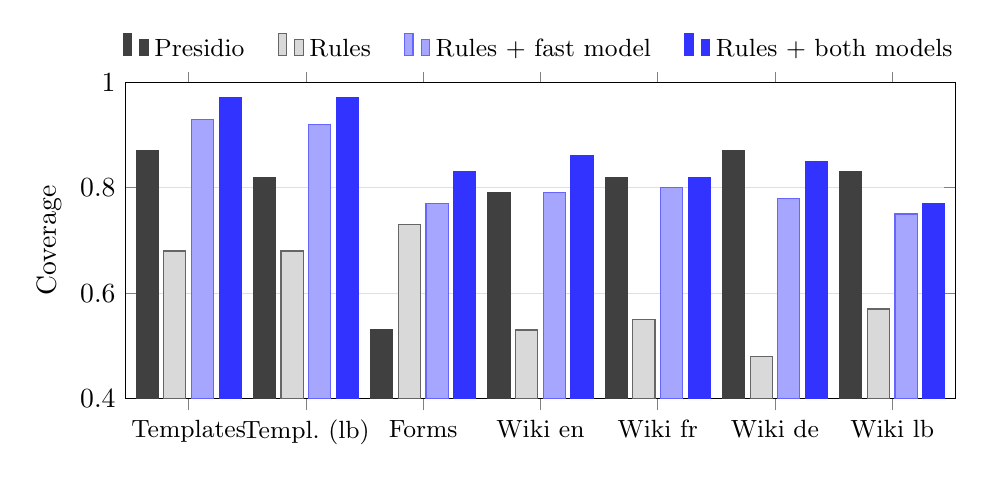
\begin{tikzpicture}
\begin{axis}[
  ybar, bar width=8pt, width=\textwidth, height=5.6cm,
  ymin=0.4, ymax=1.0, ylabel={Coverage},
  symbolic x coords={Templates,Templ.\ (lb),Forms,Wiki en,Wiki fr,Wiki de,Wiki lb},
  xtick=data, x tick label style={font=\small},
  enlarge x limits=0.09,
  legend style={at={(0.5,1.03)}, anchor=south, legend columns=4, font=\small, draw=none,
    /tikz/every even column/.append style={column sep=10pt}},
  ymajorgrids, grid style={gray!25},
]
\addplot[fill=black!75, draw=black!75] coordinates {(Templates,0.87) (Templ.\ (lb),0.82) (Forms,0.53) (Wiki en,0.79) (Wiki fr,0.82) (Wiki de,0.87) (Wiki lb,0.83)};
\addplot[fill=black!15, draw=black!60] coordinates {(Templates,0.68) (Templ.\ (lb),0.68) (Forms,0.73) (Wiki en,0.53) (Wiki fr,0.55) (Wiki de,0.48) (Wiki lb,0.57)};
\addplot[fill=blue!35, draw=blue!60] coordinates {(Templates,0.93) (Templ.\ (lb),0.92) (Forms,0.77) (Wiki en,0.79) (Wiki fr,0.80) (Wiki de,0.78) (Wiki lb,0.75)};
\addplot[fill=blue!80, draw=blue!80] coordinates {(Templates,0.97) (Templ.\ (lb),0.97) (Forms,0.83) (Wiki en,0.86) (Wiki fr,0.82) (Wiki de,0.85) (Wiki lb,0.77)};
\legend{Presidio, Rules, Rules + fast model, Rules + both models}
\end{axis}
\end{tikzpicture}
\caption{Coverage on held-out data. For the letters and forms the mean over English, French and
German is shown.}
\label{fig:coverage}
\end{figure*}

\subsection{Over-redaction and runtime}

On the 80 entity-free sentences Presidio marked 71 spans that were neither dates nor times, and
tagging marked 10 to 16 depending on the mode. On the 120 everyday sentences the counts were 115
against 2 to 12. GLiNER on its own, without rules and filters, marked 92 and 151 spans on the same
two sets. On Wikipedia sentences, 18\% of the spans Presidio marked touched no labelled entity,
against 3\% to 8\% for tagging.

The rules processed 1{,}000 words in about 4~ms. The fast mode took 0.09~s when texts were passed
in one batch, GLiNER 7.8~s, and Presidio 0.43~s with one call per text.

\section{Discussion}

The first question can be answered with a qualified yes. With a model switched on, the system
covered more than Presidio on text in Luxembourg's formats and on forms, and it marked far less of
the text that held no personal data. The advantage has identifiable sources: check digits for
local identifiers, a reader for labelled fields, and the list of everyday words. The last of these
matters most for Luxembourgish, where the dictionary reduced the wrong hits on everyday sentences
from nine to one.

The same filter explains where the system fell behind. An organisation whose name consists of
dictionary words is dropped together with the plumbers and fire brigades, and in German and
Luxembourgish, where every noun is capitalised, no rule based on capitals can tell the two apart.
Presidio keeps both, which gives it higher coverage on Wikipedia sentences and many more wrong
hits elsewhere. Which trade is better depends on the use: a leak is costly, but a text in which
every third noun is blacked out will not be used.

The answer to the second question is a warning. A test set generated from frequent real names is
largely contained in word lists built from Wikidata, even though the lists were not built from the
test set. The rules scored 0.98 on persons and fell to 0.54 when the names changed. Reporting only
the first number would have been wrong by a wide margin. Replacing the entities of an existing
test set is a cheap check that is advisable for any system that relies on lists.

\paragraph{Limitations.} The comparison is not equally fair in all rows. The rules for form fields
and identifiers were developed on a different sample of the same dataset that served as a test, so
they fit its format, although development and test coverage agreed (0.63 and 0.61 to 0.64 for the
rules in the default configuration). WikiANN, in turn, resembles the training data of spaCy's
pipelines, on which Presidio relies. Presidio can be extended with custom recognisers, and none
were written here. The everyday sentences were written by the developer, and WikiANN's labels are
produced automatically and contain errors. Most importantly, no real document was used: every
number comes from synthetic or encyclopedic text. At a recall of 0.92 per name, a document with
ten names would still leak at least one of them in more than half of all cases, so the system
should not be relied on for anonymisation without a check on the documents in question.

\section{Conclusion}

A system that validates what has a format, looks up what is listed and asks a model only for the
rest can exceed a general tool on text in Luxembourg's languages and formats while marking a
fraction of the text that contains no personal data. It does not exceed it everywhere: names made
of everyday words in German and Luxembourgish remain the open problem, and the accurate model is
slow on a CPU. The most useful methodological result is that a test set can be saturated by word
lists without any deliberate leak, and that replacing its entities exposes this at little cost.
The next step is an evaluation on real letters, emails and forms from an organisation in
Luxembourg, labelled by hand, followed by a recogniser for Luxembourgish organisations that does
not depend on capitals.

\section*{Acknowledgements}

The word lists rely on Wikidata and on the L\"etzebuerger Online Dictionnaire, both published
under CC0, and on Wikipedia text. The project was vibe coded: the software, the experiments
and a first draft of this text were produced with an AI coding assistant (Claude, Anthropic)
under the author's direction. No funding was received for this work.

\section*{Data and code availability}

Code, word lists, the template data and all result files are available at
\url{https://github.com/YannKleees/tagging}. The external datasets are downloaded by the
evaluation scripts and are not redistributed.

\bibliographystyle{unsrtnat}
\bibliography{references}

\end{document}
